%----------------------------------------------------------------------------------------
\chapter{Introduction to HPX}
%----------------------------------------------------------------------------------------
HPX (High Performance ParalleX) is a general purpose C++ runtime system for parallel and distributed applications of any scale. It strives to provide a unified programming model which transparently utilizes the available resources to achieve unprecedented levels of scalability.  This library strictly adheres to the C++14 Standard and leverages the Boost C++ Libraries which makes HPX easy to use, highly optimized, and very portable. These are the most notable features of HPX:
\vspace{0.25cm}
\begin{itemize}
\item HPX exposes a uniform, standards-oriented API for ease of programming parallel and \textcolor{azure}{distributed} applications.
\item HPX provides unified syntax and semantics for \textcolor{azure}{local and remote} operations.
\item HPX exposes a uniform, flexible, and extendable \textcolor{azure}{performance counter framework}~\cite{grubel2016dynamic,grubel2016using} which can enable runtime adaptivity
\item HPX has been designed and developed for systems of \textcolor{azure}{any scale}, from hand-held devices to very large scale systems (Raspberry Pi, Android, Server, up to super computers~\cite{daiss2019piz,heller2019harnessing}).
\end{itemize}
\vspace{0.25cm}
For a brief overview of HPX, we refer to~\cite{heller2017hpx,Kaiser2020} and for a detailed overview, we refer to~\cite{heller2019extending}. For more details about asynchronous many-task systems (AMT), we refer to~\cite{thoman2018taxonomy}.

%----------------------------------------------------------------------------------------
\subsection{Using HPX}
\label{sec:hpx:using}
%----------------------------------------------------------------------------------------
Let us look into HPX's hello world example. We have to ways to initialize the HPX runtime system. First way is to include the header \cpp{#include <hpx/hpx_main.hpp>}, see Listing~\ref{code:hpx:main}. In that case, the only thing we have to add is the new header file. Note that this header file should be the first one to be included. Before we can call the first HPX function, the HPX runtime system needs to be initialized. Second way is to include the header \cpp{#include <hpx/hpx_init.hpp>}, see Listing~\ref{code:hpx:init}. In that case, the \cpp{hpx_main} function is defined in Line~4 and we place the code as we like to have in the \cpp{main} function there and use \cpp{hpx::finalize()} as the return value to make sure the HPX runtime system is stopped. To initialize the HPX runtime system, the function \cpp{hpx::init(argc, argv)} has to be called. Note that this header file should be the first one to be included. All HPX functions have to be called within the \cpp{hpx_main} function to make sure the HPX runtime system is initialized. \\

Assuming that HPX is installed on the system, we need to provide some compiler and linker flags to compile the HPX application. Note that on Fedora one can install HPX by using \bash{sudo dnf install hpx-devel} or using this
tutorial\link{https://www.diehlpk.de/blog/hpx-fedora/}. Listing~\ref{code:cmake:hpx} shows a example \textit{CMakeLists.txt} file to compile the programs shown in Listing~\ref{code:hpx:main} or Listing~\ref{code:hpx:init}. For more details about CMake, we refer to Section~\ref{sec:cmake}. Listing~\ref{code:cmake:compile:hpx} shows how to compile the program and run it. Note that the command line option \cpp{--hpx:threads} specifies how many CPUs HPX is allowed yo use. 


\begin{lstlisting}[language=c++,caption={Initializing the HPX runtime system (I).\label{code:hpx:main}},float,floatplacement=tb]
#include <hpx/hpx_main.hpp>
#include <iostream>

int main()
{
    std::cout << "Hello World!\n" << std::endl;
    return 0;
}
\end{lstlisting}


\begin{lstlisting}[language=c++,caption={Initializing the HPX runtime system (II).\label{code:hpx:init}},float,floatplacement=tb]
#include <hpx/hpx_init.hpp>
#include <iostream>

int hpx_main(int, char**)
{
    // Say hello to the world!
    std::cout << "Hello World!\n" << std::endl;
    return hpx::finalize();
}

int main(int argc, char* argv[])
{
    return hpx::init(argc, argv);
}
\end{lstlisting}


\begin{minipage}{\linewidth}
\begin{minipage}{0.45\linewidth}
\begin{lstlisting}[language=bash,caption={Content of the CMakeLists.txt to build HPX applications.\label{code:cmake:hpx}},emph={project, add_executable,cmake_minimum_required},emphstyle={\color{azure}\bfseries}]
cmake_minimum_required(VERSION 3.3.2)
project(my_hpx_project CXX)
find_package(HPX REQUIRED)
add_hpx_executable(my_hpx_program
    SOURCES main.cpp
)
\end{lstlisting}
\end{minipage}
\hfill
\begin{minipage}{0.45\linewidth}
\begin{lstlisting}[language=bash,caption={Build instructions for CMake.\label{code:cmake:compile:hpx}}]
cmake .
make
./my_hpx_program --hpx:threads=4
\end{lstlisting}
\end{minipage}
\end{minipage}



%----------------------------------------------------------------------------------------
\section{Parallel algorithms}
\index{algorithms!parallel}
\index{parallel algorithms}
\index{HPX!parallel algorithms}
%----------------------------------------------------------------------------------------
In Section~\ref{sec:stl:parallel:algorithms} we looked at the experimental parallel algorithms provided by the C++ STL. HPX provides the parallel algorithms as well and the API is identical and we just need to replace the \cpp{std} name space with \cpp{hpx} name space. Recall the example in Listing~\ref{code:parallel:algorithms} and now we implement the same example using HPX's parallel algorithms. Listing~\ref{code:hpx:parallel:reduce} shows how to compute the sum of the elements in the vector \cpp{values} parallel. Note that solely had to replace \cpp{std::execution::par} by HPX's name space which is a little bit different and reads as \cpp{hpx::execution::par}. The same for \cpp{std::reduce} and this name space reads as \cpp{hpx::ranges::reduce}\link{https://hpx-docs.stellar-group.org/latest/html/libs/algorithms/api.html?highlight=reduce\#\_CPPv3N3hpx8parallel2v16reduceERR8ExPolicy8FwdIterB8FwdIterE1TRR1F}. Until now the API is equal to the one of the C++ STL. Now, we look into the additional features provided by HPX. First, we look into the additional features for execution policies\index{HPX!execution policies}. In Line~16 we specify a dynamic chunk size \cpp{dynamic_chunk_size} and pass this execution policy to the execution policy using \cpp{.with(scs)}. Following execution parameters are provided:
\vspace{0.25cm}
\begin{itemize}
\item \lstinline|hpx::execution::static_chunk_size|\link{https://hpx-docs.stellar-group.org/latest/html/libs/execution/api.html?highlight=static\_chunk\_size\#\_CPPv3N3hpx8parallel9execution17static\_chunk\_sizeE} \\
Loop iterations are divided into pieces of a given size and then assigned to threads.
\item \lstinline|hpx::execution::auto_chunk_size|\link{https://hpx-docs.stellar-group.org/latest/html/libs/execution/api.html?highlight=auto\_chunk\_size\#\_CPPv3N3hpx8parallel9execution15auto\_chunk\_sizeE} \\
Pieces are determined based on the first 1\% of the total loop iterations. 
\item \lstinline|hpx::execution::dynamic_chunk_size|\link{https://hpx-docs.stellar-group.org/latest/html/libs/execution/api.html?highlight=dynamic\_chunk\_size\#\_CPPv3N3hpx8parallel9execution18dynamic\_chunk\_sizeE} \\
Dynamically scheduled among the cores and if one core finished it gets dynamically assigned a new chunk.
\end{itemize}
\vspace{0.25cm}
For more details, we refer to~\cite{grubel2015performance}. Another possibility is to use machine learning techniques for choosing the chunk size. For more details, we refer to~\cite{shirzad2019scheduling}. Second, in HPX once can obtain a future from a parallel for loop and us it for synchronization. In Line~23 of Listing~\ref{code:hpx:parallel:reduce} shows how to obtain a future with the result of the reduce operation by adding the expression \cpp{hpx::execution::task} as an argument to the execution policy. Now we can use the parallel for loops and combined them with the future for asynchronous programming. Note that currently these features are only available yet in HPX. Third, HPX provides range-based for loops\link{https://hpx-docs.stellar-group.org/latest/html/manual/writing_single_node_hpx_applications.html?highlight=parallel\_for\_loop} which is neat for iteration over the elements of a vector using the index and not the vector element itself. Listing~\ref{code:hpx:parallel:range:loop} shows how to use a range-based parallel for loop to print the vector's element to the standard output stream.  The second function argument is the first value of the vector, the third one the vector's length, and the fourth argument is a Lambda function, see Section~\ref{sec:lambda:function}. The first argument of the Lambda function is the index of the the vector to be processed in the range of \cpp{0} and \cpp{values.size()}.


\begin{lstlisting}[language=c++,caption={Parallel algorithms (reduce) using HPX.\label{code:hpx:parallel:reduce}},float,floatplacement=tb]
#include <hpx/hpx_init.hpp>
#include<hpx/include/parallel_reduce.hpp>

int main()
{

std::vector<double> values = {1,2,3,4,5,6,7,8,9};

// HPX parallel algorithms
std::cout<< hpx::ranges::reduce(hpx::execution::par,
	values.begin(),
	values.end(),
	0);
	
// HPX parallel algorithms using execution policies
hpx::execution::dynamic_chunk_size scs(10);
std::cout<< hpx::ranges::reduce(hpx::execution::par.with(cs),
	values.begin(),
	values.end(),
	0);
	
// HPX parallel algorithms returning a future
auto f = hpx::ranges::reduce(
	hpx::execution::par(hpx::execution::task),
	values.begin(),
	values.end(),
	0);

std::cout<< f.get();
  
return EXIT_SUCCESS;
}

\end{lstlisting}

\begin{lstlisting}[language=c++,caption={Parallel range-based for loops using HPX.\label{code:hpx:parallel:range:loop}},float,floatplacement=tb]
#include <hpx/hpx_init.hpp>
#include<vector>
#include<iostream>
#include<hpx/include/parallel_for_loop.hpp>

int main()
{

std::vector<double> values = {1,2,3,4,5,6,7,8,9};

hpx::for_loop(
	hpx::execution::par, 
	0, 
	values.size();
	[](boost::uint64_t i)
		{
		std::cout<< values[i] << std::endl;
		}
	);

return EXIT_SUCCESS;
}

\end{lstlisting}

%----------------------------------------------------------------------------------------
\section{Asynchronous programming}
\label{sec:hpx:async}
\index{future}
\index{async}
\index{HPX!asynchronous programming}
%----------------------------------------------------------------------------------------
HPX provides the same features as the C++ language for asynchronous programming, see Chapter~\ref{sec:async:coding} for more details. In this section, we show how to use HPX's function instead of \cpp{std::future} and \cpp{std::async}, since HPX provides more flexibility here. As a disclaimer this is really easy, since we can use the code of the previous example and just replace the name space \cpp{std} with the name space \cpp{hpx}. Listing~\ref{code:hpx:future} shows an example of the example for computing the square number of a asynchronously. In Line~2 the header \cpp{#include <hpx/incldue/lcos.hpp>} is needed to use \cpp{hpx::future} and \cpp{hpx::async}\link{https://stellar-group.github.io/hpx/docs/sphinx/latest/html/examples/fibonacci_local.html?highlight=async}. In Line~12 the function \cpp{square} is called asynchronously using \cpp{hpx::async(square,10)}. Note that the first argument is the name of the function and the second one the function argument. The function call return a \cpp{hpx::future<int>} since the return type of the function is \cpp{int}. To access the result of the function, if the computation has finished the function \cpp{.get()} is used. Note that the only difference here is not to include the header \cpp{#include <future>} and use \cpp{hpx::future} instead of \cpp{std::future} and same for \cpp{hpx:async} instead of \cpp{std::async}. Thus, it is really easy to switch between HPX and C++ for asynchronous programming.

\begin{lstlisting}[language=c++,caption={Asynchronous computation of the square number using HPX.\label{code:hpx:future}},float,floatplacement=tb]
#include <hpx/hpx_init.hpp>
#include <hpx/incldue/lcos.hpp>
#include <iostream>

int square(int a)
{ 
    return a*a; 
}

int main()
{
    hpx::future<int> f1 = hpx::async(square,10); 
    
    std::cout << f1.get() << std::endl;
    
    return EXIT_SUCCESS;
}

\end{lstlisting}

\begin{exercise}
Write the program in Listing~\ref{code:async:taylor} using \cpp{hpx::future} and \cpp{hpx::async}.
\end{exercise}

The benefit of using HPX is that more features for the synchronization of future is provided. In Listing~\ref{code:hpx:future:sync} some of these functionality is shown. In Line~1 a \cpp{std::vector} holding the \cpp{hpx::future<int>} is declared. In Lines~2--3 two futures of the two asynchronous function class are pushed to the vector. In Line~6 the expression \cpp{hpx::when_all} is used to make a barrier which waits until all computations of the asynchronous launched functions are ready. By calling \cpp{.then()} we specify what is done if all futures are ready. To do so, we provide a lambda function, see Section~\ref{sec:lambda:function}, which has a future with the \cpp{std::vector} of futures as its argument. In Line~7 we use the function \cpp{.get()} and this future to get the \cpp{std::vector} of futures. In line~7 and Line~8, we print the results as usual. Following synchronization options\link{https://stellar-group.github.io/hpx/docs/sphinx/latest/html/terminology.html\#term-lco} are available:
\begin{itemize}
\item \cpp{hpx::when_all} \\
It \textit{AND}-composes all the given futures and returns a new future containing all the given futures.
\item \cpp{hpx::when_any} \\
It \textit{OR}-composes all the given futures and returns a new future containing all the given futures.
\item \cpp{hpx::when_each} \\
It \textit{AND}-composes all the given futures and returns a new future containing all futures being ready.
\item \cpp{hpx::when_some} \\
It \textit{AND}-composes all the given futures and returns a new future object representing the same list of futures after n of them finished.
\end{itemize}



\begin{lstlisting}[language=c++,caption={Advanced synchronization of futures using HPX.\label{code:hpx:future:sync}},float,floatplacement=tb]
std::vector<hpx::future<int>> futures;

futures.push_back(hpx::async(square,10);
futures.push_back(hpx::async(square,100);

hpx::when_all(futures).then([](auto&& f){
 auto futures = f.get();
 std::cout << futures[0].get() 
 	<< " and " << futures[1].get();
});
\end{lstlisting}

%----------------------------------------------------------------------------------------
\subsection{Advanced asynchronous programming}
\label{sec:hpx:advanced:sync}
%----------------------------------------------------------------------------------------
HPX provides additional features for asynchronous programming which are not yet in the C++ standard. In this section, we look into these. Therefore, we look into the \cpp{struct stepper} of the serial version, see Listing~\ref{code:heat:central:difference}, and add futures to have asynchronous execution of the solver for the one-dimensional heat equation. Listing~\ref{code:hpx:future:ready} shows the new \cpp{struct stepper} using futures. The first change is that the type \cpp{partition}, which was a simple \cpp{double} value before, is replaced by \cpp{hpx::shared_future}\index{future!shared}. Note that the \cpp{hpx::lcos::future} has the exclusive ownership model and if the future is out of scope, it will be not available anymore. To avoid the out of scope situation, the \cpp{hpx::shared_future} has the reference counting ownership model. Here, all references to the object are counted and the object solely goes out of scope if there are zero references. These concepts are equal to \cpp{std::unique_ptr}\link{https://en.cppreference.com/w/cpp/memory/unique_ptr} and \cpp{std::shared_ptr}\link{https://en.cppreference.com/w/cpp/memory/shared_ptr}.\\
 
The first feature is the keyword \cpp{hpx::make_ready_future}\link{https://hpx-docs.stellar-group.org/latest/html/api.html?highlight=make_ready_future}\index{future!ready}, see Line~22 of Listing~\ref{code:hpx:future:ready}. Since the \cpp{partition} is now a \cpp{hpx::shared_future} the boundary conditions and initial conditions have to be a future too. However, since these are constant values and no computation is needed the future is immediately ready. Since HPX does not know that there is no execution, we can use a \cpp{hpx::make_ready_future} ready to propagate this information to the asynchronous execution tree.\\

Second, since we use futures for the \cpp{partition}, but the function to evaluate the central difference \cpp{heat(double left, double middle, double right)} takes \cpp{double} values as arguments. We either have to change the function to take futures as its arguments and call the \cpp{.get()} function inside. To avoid these two things, HPX provides the so-called unwrapping of a function with the keyword \cpp{hpx::util::unwrapping}\index{HPX!unwrapping}. In Line~24 of Listing~\ref{code:hpx:future:ready} the function \cpp{heat} is unwrapped and the function \cpp{Op} takes futures as its arguments. So In Line~37 of the \cpp{hpx::launch::async} we can pass the \cpp{current} elements which are of the type \cpp{hpx::shared_future<double>} to a function which assumes \cpp{double values}.\\

Third, HPX has the keyword \cpp{hpx::dataflow}\index{HPX!dataflow} to use unwrapping for the combination of \cpp{hpx::when_all} and \cpp{.then}. Imagine you have a vector \cpp{std::vector<hpx::lcos::future<int>> futures;} and pass it to \cpp{hpx::when_all(futures).then([](auto&& f)\{\});} the vector \cpp{futures} will be wrapped in the future \cpp{auto&& f}. SO if we want to access the elements of the vector we have to call \cpp{f.get()}. An easier approach is to use \cpp{hpx::dataflow} as it is done in Line~36 in Listing~\ref{code:hpx:future:ready}. The first argument is \cpp{hpx::launch::async} to launch asynchronous and a future is returned. Another possibility is to use \cpp{hpx::launch::sync} to launch synchronous. The second argument is the unwrapped function of the \cpp{heat} function, see Line~24. The last three remaining arguments are the futures with the values for the central difference scheme evaluation. Before we can return the current solution, we have to call \cpp{hpx::when_all} to synchronous all futures of the current solution.\\

Figure~\ref{fig::stencil:benchmark:1} shows the execution time of the serial vs the asynchronous implementation for 1 CPU. We clearly see that the execution time even for one CPU is lower. Figure~\ref{fig::stencil:benchmark:2} shows the execution time for various amount of CPUs for the asynchronous implementation. Here, we can see that for enough grid points the we get some benefit for adding more CPUs which means we have to have enough work to keep the CPUs busy. To obtain better results, we have to extend the code to control its granularity.

\begin{lstlisting}[language=c++,caption={Futurized version of the one-dimensional heat equation.\label{code:hpx:future:ready}},float,floatplacement=tbp]
struct stepper
{
    // Our partition type
    typedef hpx::shared_future<double> partition;

    // Our data for one time step
    typedef std::vector<partition> space;

    // do all the work on 'nx' data points for 'nt' time steps
    hpx::future<space> do_work(std::size_t nx, std::size_t nt)
    {
        using hpx::dataflow;
        using hpx::util::unwrapping;

        // U[t][i] is the state of position i at time t.
        std::vector<space> U(2);
        for (space& s : U)
            s.resize(nx);

        // Initial conditions: f(0, i) = i
        for (std::size_t i = 0; i != nx; ++i)
            U[0][i] = hpx::make_ready_future(double(i));

        auto Op = unwrapping(&stepper::heat);

        // Actual time step loop
        for (std::size_t t = 0; t != nt; ++t)
        {
            space const& current = U[t % 2];
            space& next = U[(t + 1) % 2];

            // WHEN U[t][i-1], U[t][i], and U[t][i+1] have been computed, THEN we
            // can compute U[t+1][i]
            for (std::size_t i = 0; i != nx; ++i)
            {
                next[i] = dataflow(
                        hpx::launch::async, Op,
                        current[idx(i, -1, nx)], current[i], current[idx(i, +1, nx)]
                    );
            }
        }

        // Return the solution at time-step 'nt'.
        return hpx::when_all(U[nt % 2]);
    }
};
\end{lstlisting}


\begin{figure}[btp]
\centering
\begin{subfigure}{.4\textwidth}
\begin{tikzpicture}
\selectcolormodel{gray}
\begin{axis}[xlabel=Grid points,ylabel=Execution time, grid=both,title=1 CPU]
\addplot table [x=Grid_Points, y=Execution_Time_sec, col sep=comma] {./data/stencil_serial.dat};
\addlegendentry{Serial}
\addplot table [x=Grid_Points, y=Execution_Time_sec, col sep=comma] {./data/stencil_2_1.dat};
\addlegendentry{Futurization}
\end{axis} 
\end{tikzpicture}
\caption{Serial vs asynchronous execution}
\label{fig::stencil:benchmark:1}
\end{subfigure}

\begin{subfigure}{.4\textwidth}
\begin{tikzpicture}
\selectcolormodel{gray}
\begin{axis}[xlabel=Grid points,ylabel=Execution time, grid=both,title= Stencil 2,legend pos=north west]
\addplot table [x=Grid_Points, y=Execution_Time_sec, col sep=comma] {./data/stencil_2_1.dat};
\addlegendentry{1 CPU}
\addplot table [x=Grid_Points, y=Execution_Time_sec, col sep=comma] {./data/stencil_2_2.dat};
\addlegendentry{2 CPU}
\addplot table [x=Grid_Points, y=Execution_Time_sec, col sep=comma] {./data/stencil_2_4.dat};
\addlegendentry{4 CPU}
\addplot table [x=Grid_Points, y=Execution_Time_sec, col sep=comma] {./data/stencil_2_6.dat};
\addlegendentry{6 CPU}
\end{axis}
\end{tikzpicture}
\caption{Execution time for various number of CPUs for the asynchronous implementation}
\label{fig::stencil:benchmark:2}
\end{subfigure}
\caption{Comparison of the serial vs asynchronous execution~(\subref{fig::stencil:benchmark:1}) and speed-up for various amount of CPUs~(\subref{fig::stencil:benchmark:2}).}
\label{fig:hpx:stencil:scaling1}
\end{figure}

%----------------------------------------------------------------------------------------
\subsection{Adding grain size control}
%----------------------------------------------------------------------------------------
In Section~\ref{heatequation:serial:grainsize} the control of the granularity was added to the serial implementation of the one-dimensional heat equation. here, we extend the code with the futurization with the grain size control. First, we extend the \cpp{struct partion_data}, see Listing~\ref{code:hpx:future:grain}. In Line~39 we change the class members to a \cpp{double []} array and we introduce \cpp{size_t size_} to the store the size of the partition. Note that we use a smart pointer \cpp{std::unique_ptr} to store the  \cpp{double []} array. The shared pointer is essential since we need to use the reference counter model to keep track that the array does not go out of scope. For more details about smart pointer we refer to Section~\ref{cpp:smart:pointer}. In the constructor, we use the expression \cpp{new double [size]} to allocate a double array od the size \cpp{size}. Fore more details about the \cpp{new} expression, we refer to Section~\ref{sec:memory:management}. \\

By adding the grain size control to futurized implementation, we see some performance improvement compared to the previous implementation, see Figure~\ref{fig:hpx:stencil:scaling1}. In Figure~\ref{fig:scaling:future:grain:size} the number of discrete nodes is fixed to $1000000$ and the grain size varies which means the amount of point inside a partition change. For using one and two CPUs, we see the typical curve for the grain size control. Using a grain size of one results in the largest execution time. First, while increasing the grain size the execution times goes down until the so-called sweet spot. At the sweet spot the execution is as its minimum and decreases after. Here, it is important to find this sweet spot which depends on various factors, \emph{e.g.}\ the computation, the algorithm, and the architecture of the hardware. So for each amount of discrete nodes one has to find the sweet spot.


\begin{lstlisting}[language=c++,caption={Adding the grain size control the futurized one-dimensional heat equation.\label{code:hpx:future:grain}},float,floatplacement=tbp]
struct partition_data
{
public:
    explicit partition_data(std::size_t size)
      : data_(new double[size])
      , size_(size)
    {
    }

    partition_data(std::size_t size, double initial_value)
      : data_(new double[size])
      , size_(size)
    {
        double base_value = double(initial_value * size);
        for (std::size_t i = 0; i != size; ++i)
            data_[i] = base_value + double(i);
    }

    partition_data(partition_data&& other) noexcept
      : data_(std::move(other.data_))
      , size_(other.size_)
    {
    }

    double& operator[](std::size_t idx)
    {
        return data_[idx];
    }
    double operator[](std::size_t idx) const
    {
        return data_[idx];
    }

    std::size_t size() const
    {
        return size_;
    }

private:
    std::unique_ptr<double[]> data_;
    std::size_t size_;
};

\end{lstlisting}

\begin{figure}[tbp]
\centering
\begin{tikzpicture}
\selectcolormodel{gray}
\begin{axis}[xlabel=Partitions,ylabel=Execution time, grid=both,title=Stencil 4,legend pos=north west]
\addplot table [x=Partitions, y=Execution_Time_sec, col sep=comma] {./data/stencil_4_1cpu_1000000.dat};
\addlegendentry{1 CPU}
\addplot table [x=Partitions, y=Execution_Time_sec, col sep=comma] {./data/stencil_4_2cpu_1000000.dat};
\addlegendentry{2 CPU}
\end{axis}
\end{tikzpicture}
\caption{Variation of grain size for fixed $1000000$ discrete nodes. For one CPU and the two CPUs, we see the typical curve where the execution time goes down, ther sweet spot is reached, and the execution increases after. }
\label{fig:scaling:future:grain:size}
\end{figure}
%----------------------------------------------------------------------------------------
\section{Semaphores}
\label{sec:hpx:semaphores}
\index{semaphores}
%----------------------------------------------------------------------------------------
In Section~\ref{sec:deadlocks} the \cpp{std::mutex}, which is tied to one thread and only one thread can lock or unlock the mutex. Now the look into a semaphore and here any thread can access the ownership on a semaphore. Note that the C++ standard does not define semaphores and they are only available suing HPX. The concept of semaphores was introduced by E. Dijkstra~\cite{dijkstra1962over} and more details are available here~\cite{downey2008little}. Before we look into the source code, we will focus on one example. \\

Imagine a public library lending books with no late fee. The library has 5 copies of the Hitckhiker's Guide to the Galaxy~\cite{adams2017ultimate}. So the first five people can borrow these copies and keep them for an infinite amount of time, since there are no late fees. Now, if person number six wants to borrow one copy, this person has to wait until one of the five borrowers return one copy. So the library assigns one of the copies to this person, but if none is waiting the copy just goes back to the shelf until one asks for it. \\

This example can be explained in C++ using a semaphore. A semaphore has two variables. First, a \cpp{maximum count} which is from the example the total amount of copies. Second, a \cpp{current count} which relates to the amount of currently borrowed copies. Now, we have the the so-called \textcolor{azure}{P-Operation} and \textcolor{azure}{V-Operation}. The \textcolor{azure}{P-Operation} is done using the \cpp{wait} function. Here the variable \cpp{current count} is decreased. If the count is $\geq$ zero then the decrement just happens and the function will return. If the count is zero the function will wait until one other thread called the \lstinline|signal| function. This is refereed to as \textcolor{azure}{P-Operation}\index{P-Operation}. If the \lstinline|signal| function is called, the current count is increased. If the count was zero before you called \lstinline|signal| function and another thread was blocked in \lstinline|wait| then that thread will be executed. If multiple threads are waiting, only one will be executed and the reaming ones have to wait for another increment of the counter. This is refereed to as \textcolor{azure}{V-Operation}\index{V-Operation}. Listing~\ref{code:hpx:semaphore} shows the usage of the semaphore in HPX. In Line~2 the semaphore is generated an the maximal count is passed as argument \cpp{nd}. In Line~5 the ownership of thread \cpp{t} is released using the P-Operation (\cpp{signal} function). In Line~8 the thread \cpp{t} obtains the ownership using the V-Operation (\cpp{wait} function).


\begin{lstlisting}[language=c++,caption={HPX's semaphores.\label{code:hpx:semaphore}},float,floatplacement=tb]
// Generate a semaphore with maximal count nd
hpx::lcos::local::sliding_semaphore sem(nd);

// Release ownership for t
sem.signal(t);

// Obtain ownership for t
sem.wait(t);
\end{lstlisting}


%----------------------------------------------------------------------------------------
\section{Distributed programming}
%----------------------------------------------------------------------------------------

%----------------------------------------------------------------------------------------
\subsection{Serialization}
\index{serialization}
%----------------------------------------------------------------------------------------
In shared memory parallelism the allocated data resits in the memory on the node, however, in the distributed memory parallelism each of the physical nodes has its own memory. If one uses \cpp{std::vector<double>} or \cpp{double[]} this is a so--called unflatten\index{serialization!unflatten} data structure representation in C++. However, this data structure can not be wrapped in a parcel and send over the network to another physical node. Before the data structure can be wrapped in a parcel, the data needs to be flatten\index{serialization!flatten} to a one-dimensional stream of bits. For the serialized stream of bits there is human-readable (text) and non-human-readable (binary) format possible. The advantage of the text variant is that the message is readable, but is larger. For the binary variant the message is might smaller, but can not be analyzed for debugging.\\

Figure~\ref{fig:sending:network} shows the protocol to send data over the network from locality 1 to locality 2. On locality 1, first the data is allocated in the local memory, for example one could allocate the vector \cpp{std::vector<double> vec = {0.0,0.5,1.0};} in the local memory of locality 1. Second, the \cpp{std::vector<double>} is serialized which means the \cpp{std::vector} is transformed in a stream of bits containing the data of the vector and some additional information, \emph{e.g.}\ the size of elements. Third, the flattened bit of streams is wrapped into a parcel which is send over the network to locality 2. For more details for sending parcels over the network, we refer to Section~\ref{sec:distributed:programming}. On the receiving locality 2, first the parcel is received and unpacked. Second, the data for the content of the parcel is allocated in the local memory of locality 2. Third, the flattened data from the received parcel is deserialized and stored in the local memory of locality 2. \\

\begin{figure}[tb]
\begin{center}
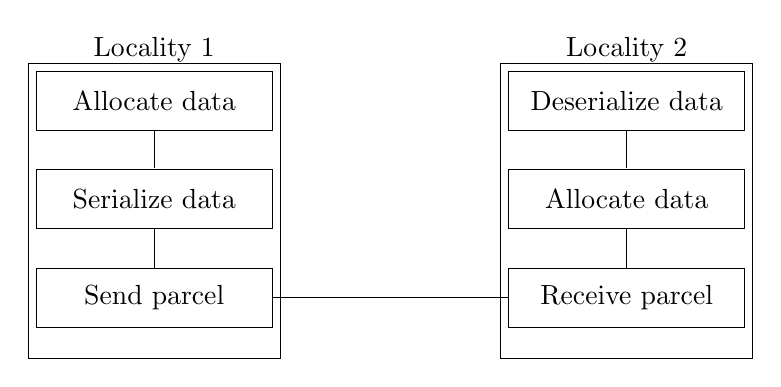
\begin{tikzpicture}
\draw (0,0) rectangle ++(3,-0.75) node[pos=.5] {Allocate data};

\draw (0,-1.25) rectangle ++(3,-.75) node[pos=.5] {Serialize data};

\draw (0,-2.5) rectangle ++(3,-.75) node[pos=.5] {Send parcel};

\draw (-0.1,0.1) rectangle ++(3.2,-3.75);

\node[above] at (1.5,0) {Locality 1};

\draw (6,0) rectangle ++(3,-0.75) node[pos=.5] {Deserialize data};

\draw (6,-1.25) rectangle ++(3,-.75) node[pos=.5] {Allocate data};

\draw (6,-2.5) rectangle ++(3,-.75) node[pos=.5] {Receive parcel};

\draw (5.9,0.1) rectangle ++(3.2,-3.75);

\node[above] at (7.5,0) {Locality 2};

\draw (1.5,-0.75) -- (1.5,-1.23) ;
\draw (1.5,-2.) -- (1.5,-2.5) ;

\draw (3,-2.875) -- (6,-2.875) ;

\draw (7.5,-0.75) -- (7.5,-1.23) ;
\draw (7.5,-2.) -- (7.5,-2.5) ;

\end{tikzpicture}
\end{center}
\caption{The communication between the localities (nodes) is handled by the so-called parcel port~\cite{kaiser2009parallex}. HPX uses MPI or libfrabric for communication between nodes.}
\label{fig:sending:network} 
\end{figure}

Before, we looked into the general concept of serialization and now we look on the implementation within HPX. In Listing~\ref{code:hpx:serialization} the data is allocated in the first three lines. To serialize the \cpp{double* data} array, first a \cpp{hpx::serialization::serialize_buffer} us used in Line~6 is defined. In Line~8 the buffer \cpp{serialize_buffer<double>} with \cpp{double} as its template argument is used, since we intend to serialize the \cpp{double* data} array. As the arguments of the constructor, we pass the pointer to the data and the size of the data. For now we ignore the third argument and just use this mode as the default mode. This is the part of the serialization which happens on locality 1. The deserialization which would happen on locality 2 is shown in Line~12, assuming we received the \cpp{serializable_data} object on locality 2. On locality 2 a pointer \cpp{data* copied_data} is used to store the deseralized data obtained by the function \cpp{.data()}. For sending and receiving parcels, we will look into components and action, in Section~\ref{sec:hpx:components:actions}.


\begin{lstlisting}[language=c++,caption={Serialization in HPX.\label{code:hpx:serialization}},float,floatplacement=tb]
// Allocation of the data
size_t size = 5;
double* data = new double[size];

// Serialization
using hpx::serialization::serialize_buffer;

serialize_buffer<double> serializable_data(
     data, size,
     serialize_buffer<double>::init_mode::reference);
     
// Deserialization
double* copied_data = serializable_data.data();
\end{lstlisting}


%----------------------------------------------------------------------------------------
\subsection{Components and Actions}
\label{sec:hpx:components:actions}
\index{components}
%----------------------------------------------------------------------------------------
For distributed computations within HPX, we need to look following features:
\begin{enumerate}
\item Components: \\
The server represents the global data and is a so-called HPX component which allows to create and access the data remotely through the global address space (AGAS)\cite{kaiser2014hpx}\index{AGAS}. 
\item Client: \\
The client represents the local and remote access to the component's data on all local or remote localities. 
\item Component action:\\
Each function of the component (server) needs to be wrapped into a component action to be remotely and locally available.
\item Plain actions: \\
Allows to wrap global (\cpp{static} functions in an action. So we can call this function remotely and locally.
\end{enumerate}



%----------------------------------------------------------------------------------------
\subsubsection{Action}
\index{action!component}
%----------------------------------------------------------------------------------------


%----------------------------------------------------------------------------------------
\subsubsection{Plain actions}
\index{action!plain}
%----------------------------------------------------------------------------------------
A plain action allows to call a \cpp{static} function locally and remotely. For a plain action, a \cpp{static} function  \cpp{square} is defined, see Listing~\ref{code:hpx:action:plain}. Note that actions can have a \cpp{return} expression, but we can not change data within the action. In Line~6 the function \cpp{square} is registered as a action with the name \cpp{square_action} using the expression \cpp{HPX_PLAIN_ACTION}\link{https://hpx-docs.stellar-group.org/latest/html/libs/actions_base/api.html?highlight=plain_action\#c.HPX_PLAIN_ACTION}.

\begin{lstlisting}[language=c++,caption={Plain actions in HPX.\label{code:hpx:action:plain}},float,floatplacement=tb]
static void square(double a){

	std::cout << a * a << std::endl;
}

// Register the plain action
HPX_PLAIN_ACTION(&square, square_action)
\end{lstlisting}

%----------------------------------------------------------------------------------------
\subsection{Receiving topology information}
%----------------------------------------------------------------------------------------
Following functions are available to receive topology information:
\begin{itemize}
\item \lstinline|hpx::find_here|\link{https://hpx-docs.stellar-group.org/latest/html/api/full_api.html?highlight=find_here\#_CPPv4N3hpx9find_hereER10error_code} \\
Get the global address of the locality the function is called on.

\item \lstinline|hpx::find_all_localities|\link{https://hpx-docs.stellar-group.org/latest/html/api/full_api.html?highlight=find_all_localities\#_CPPv4N3hpx19find_all_localitiesER10error_code} \\
Get the global addresses of all available localities.

\item \lstinline|hpx::find_remote_localities|\link{https://hpx-docs.stellar-group.org/latest/html/api/full_api.html?highlight=find_remote_localities\#_CPPv4N3hpx22find_remote_localitiesER10error_code} \\
Get the global addresses of all available remote localities.

\item \lstinline| hpx::get_num_localities|\link{https://hpx-docs.stellar-group.org/latest/html/libs/runtime_local/api.html?highlight=get_num_localities\#_CPPv4N3hpx18get_num_localitiesEv} \\
Get the number of all available localities.

\item \lstinline|hpx::find_locality|\link{https://hpx-docs.stellar-group.org/latest/html/api/full_api.html?highlight=find_locality\#_CPPv4N3hpx13find_localityEN10components14component_typeER10error_code} \\
Get the global address of any locality hosting the component.

\item \lstinline|hpx::get_colocation_id|\link{https://hpx-docs.stellar-group.org/latest/html/api/full_api.html?highlight=hpx\%20get_colocation_id\#_CPPv4N3hpx17get_colocation_idERKN6naming7id_typeE} \\
Get the locality hosting the object with the given address.
\end{itemize}


%----------------------------------------------------------------------------------------
\section{Overview of HPX headers}
%----------------------------------------------------------------------------------------
This section recaps some of the HPX headers and the functionality they provide. For a overview of all HPX headers, we refer to HPX's documentation~\link{https://hpx-docs.stellar-group.org/latest/html/libs/include/api.html}.
\begin{itemize}
\item \cpp{#include <hpx/hpx_main.hpp>} \\
This header includes the HPX run time systems and has to be always the first HPX header to be included. This header provides a way to initialize the HPX runtime system, see Listing~\ref{code:hpx:main}. For more details, we refer to Section~\ref{sec:hpx:using}. 

\item \cpp{#include <hpx/hpx_init.hpp>} \\
This header includes the HPX run time systems and has to be always the first HPX header to be included. This header provides a different way to initialize the HPX runtime system, see Listing~\ref{code:hpx:init}. For more details, we refer to Section~\ref{sec:hpx:using}.

\item \cpp{#include <hpx/include/locs.hpp>} \\
This header provides for example \cpp{hpx::future} (\cpp{#include <hpx/future.hpp>}) and \cpp{hpx::async} (\cpp{#include <hpx/include/future.hpp>}) functionality. Fore more details, we refer to Section~\ref{sec:hpx:async}. In addition, the advanced synchronization features, see Section~\ref{sec:hpx:advanced:sync}, are included in this header as well.

\item \cpp{#include <hpx/algorithm.hpp>} \\
This header provides the functionality of the parallel algorithms and compares to \cpp{#include <algorithm>}.
\begin{itemize}
\item \cpp{#include <hpx/include/parallel_for_loop.hpp>}
This header includes the method \cpp{hpx::for_loop} functionality, see Listing~\ref{code:hpx:parallel:range:loop}. Note if you intend to use multiple parallel algorithms, you could use \cpp{#include <hpx/algorithm.hpp>} which compares to \cpp{#include <algorithm>}.
\item \cpp{#include <hpx/include/parallel_reduce.hpp>} \\
This header includes the method \cpp{hpx::ranges::reduce} functionality which is comparable to the \cpp{std::reduce}, see Listing~\ref{code:hpx:parallel:reduce}. Note if you intend to use multiple parallel algorithms, you could use \cpp{#include <hpx/algorithm.hpp>} which compares to \cpp{#include <algorithm>}. 
\end{itemize}

\item \cpp{#include <hpx/modules/synchronization.hpp>} \\
This header provides the \cpp{hpx::lcos::local::sliding_semaphore}, see Listing~\ref{code:hpx:semaphore}. Fore more details, we refer to Section~\ref{sec:hpx:semaphores}. 

\item \cpp{#include <hpx/include/actions.hpp>} \\
This header provides the functionality for actions which we need for distributed programming, see Section~\ref{sec:hpx:components:actions}.

\item \cpp{#incldue <hpx/include/components.hpp>} \\
Provides the he functionality for the components which we need for the distributed programming, see Section~\ref{sec:hpx:components:actions}.

\item \cpp{#include <hpx/include/dataflow.hpp>} \\
Provides \cpp{hpx::dataflow::dataflow}, see for example Listing~\ref{code:hpx:future:ready}.
\end{itemize}

\newpage
\theendnotes